\subsection{System Implementation}
The idea of the implementation is to create a light bulb connected to the cloud with pre-processing on the edge. Every time the light bulb is turned on or off the IoT device sends the status to the gateway. The gateway then creates a usage pattern and sends this statistics in intervals to the cloud for further processing and storage. This enables automated maintenance and more. The orchestration and management of the gateway and IoT device is done in the cloud where the light bulb can be controlled as well.

To reduce the overall system complexity only one device is deployed at each network layer. The architecture is shown in \cref{fig:actualSetup}. The IoT device, a esp32, is connected to a button and a light, the RPi makes up the edge layer and the VPS the cloud layer.
\begin{figure}[!ht]
    \centering
    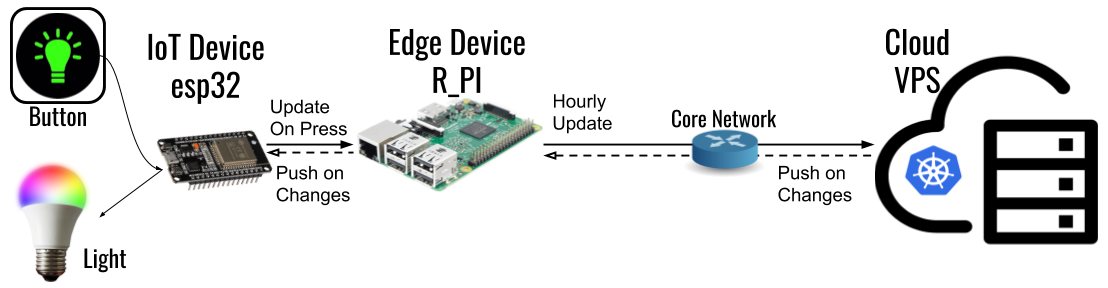
\includegraphics[width=\textwidth]{figures/actualSetup.png}
    \caption{The Implemented Hardware Architecture}
    \label{fig:actualSetup}
\end{figure}
On the edge, all devices are directly connected either through wire or WiFi and are only dependent on each other to provide the normal functions. The expected round trip time (RTT) for a given signal should be rather low translating into an immediate response. In more extensive examples, the RPi could first check if pressing the button is even permissible and only then turn on the light/machine etc. In \cref{fig:actualSetup} the solid arrows stand for communication instantiated by the system and the dashed arrows communication instantiated by external changes. The systems internal communication normally goes up, from the IoT devices to the cloud, whereas system external communication goes the other way around. It is also expected that the system internal communication happens far more frequently than the system external one.

\Cref{fig:actualImplementationSetup} uses the same layout as \cref{fig:implementationSetup} but shows the actual system implementation. Comparing it to the desired system under \cref{sec:desiredSystem} shows that major and minor changes following the classification of the requirements had to be made as technology and time did not allow for a full implementation.

\begin{figure}[!ht]
    \centering
    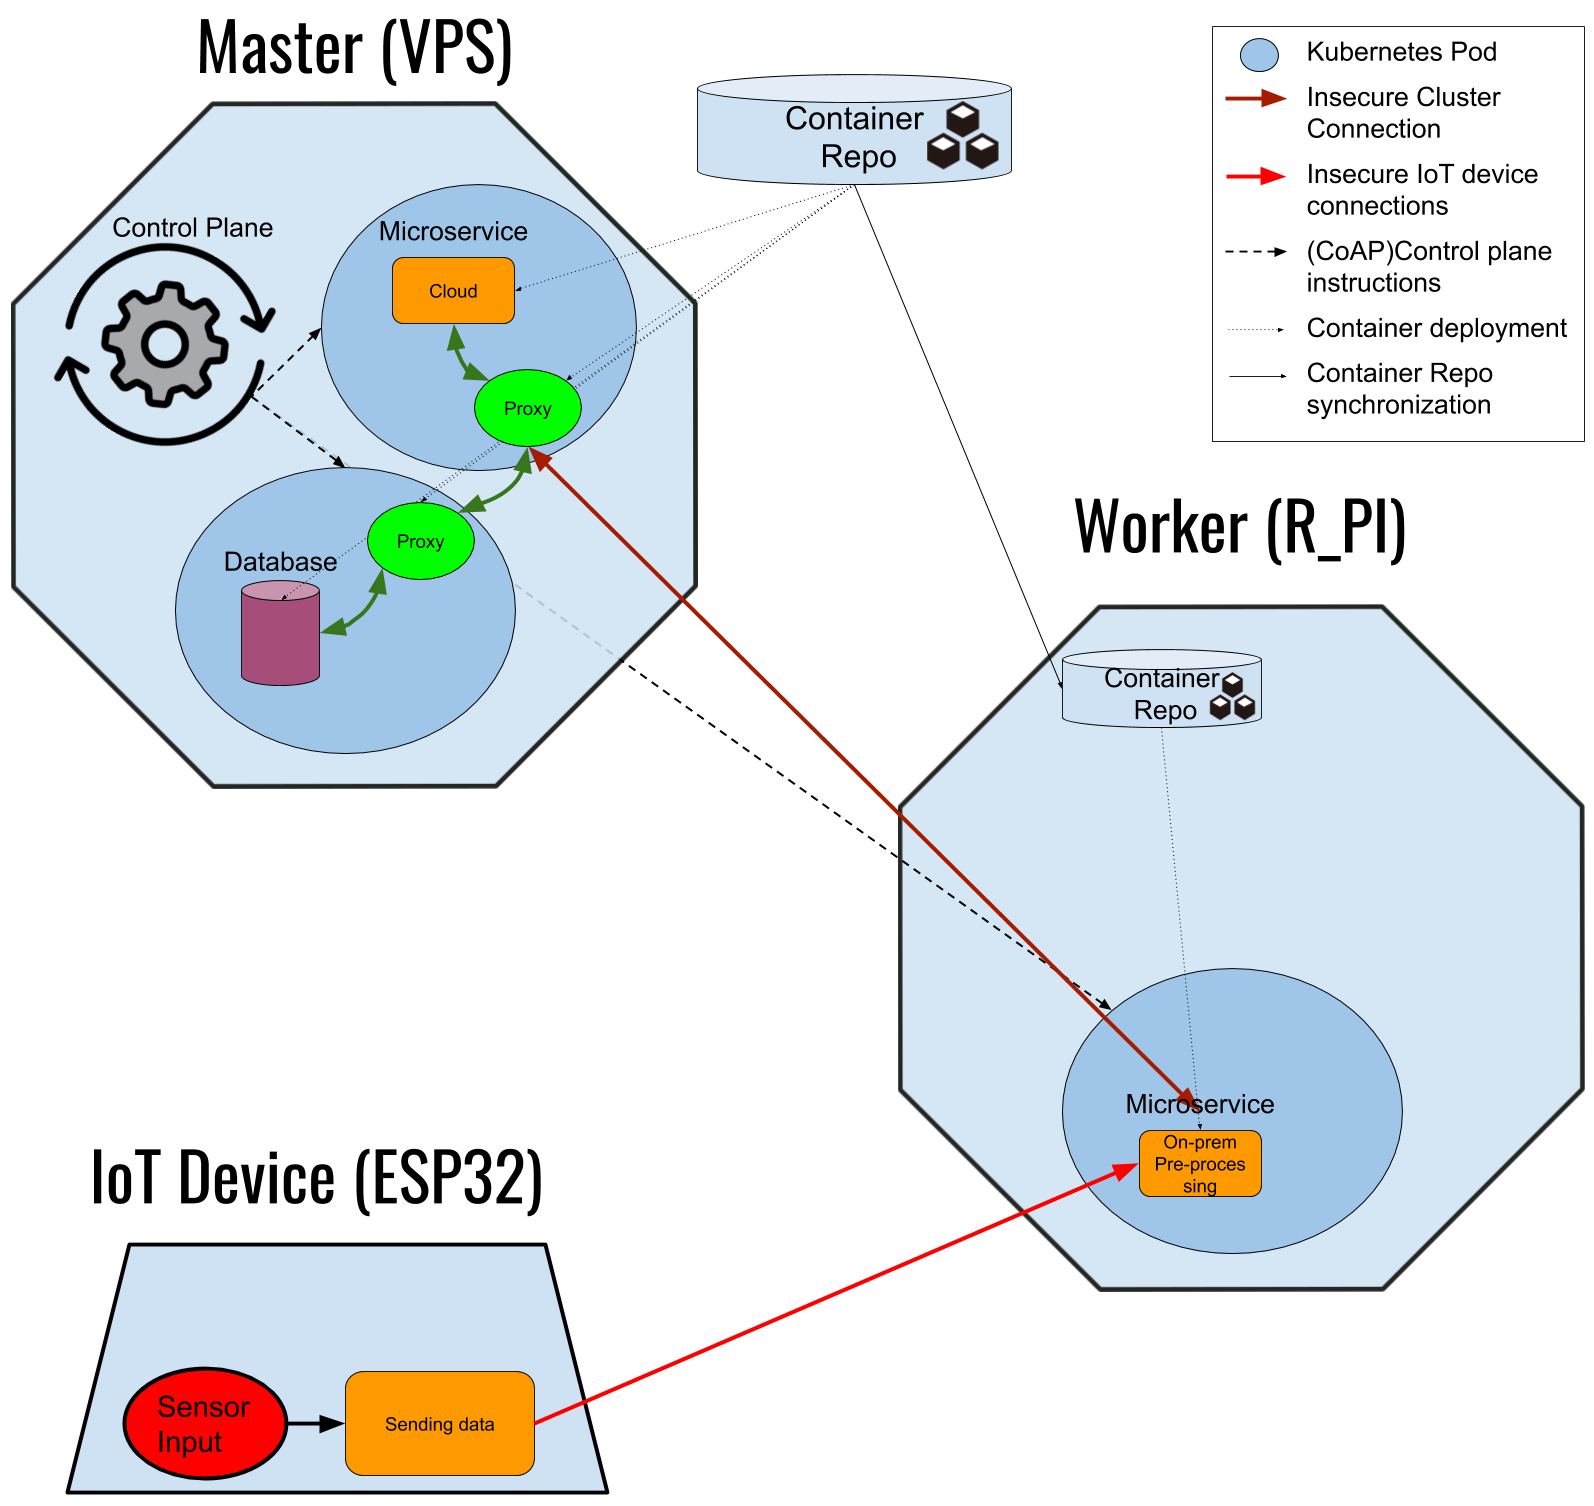
\includegraphics[width=\textwidth]{figures/actualImplementationSetup.png}
    \caption{The Actual System Architecture}
    \label{fig:actualImplementationSetup}
\end{figure}

The cloud part is unchanged from the desired setup. The edge part had to be adopted due to technical issues. The Istio envoy proxy does not compile for the ARM architecture yet. Istio provides traffic shaping and routing, default mutual TLS encryption between services, an extensive ingress gateway and more. Kubernetes is already capable of some of these things but Istio is a far more potent tool. Its absence makes it impossible to reroute network traffic from the application to another destination and importantly the traffic between the edge and the cloud will not be encrypted. At the time of writing the Istio team is working on a patch for ARM devices. Using human produced certificates as an alternative is not a good idea, especially for small project as the certificates have to be kept up to date, should be rotated and mutual TLS is hard to implement.

Similarly, the CoAP librarby for esp32 does not support DTLS yet. The developers are aware of it and are working on fixing it. Protobufs are base 128 encode message which provides a shielding against to most rudimentary attacks, but it is not a security mechanism. Finally, due to time issues and prioritization the update service for the IoT device was not implemented.

Apart from the automatic updates for the edge device, the networking and encryption issues, all requirements labeled as SHOULD or MUST have been successfully implemented. By pressing a button a user can turn on or off a light. In the background, this data is sent from the esp32 to the RPi, which processes the data and sends a usage statistic of the light usage in defined time intervals to the server for further processing and storage. The system can also change the state of the light automatically from a centralized input field. Further, the administrator can update the specifications for all cluster internal resources (edge or cloud) and the system works towards implementing this specifications. It also means, in case of failure, e.g. an application crash on the edge, the system can reschedule this application. 

\begin{figure}[!ht]
    \centering
    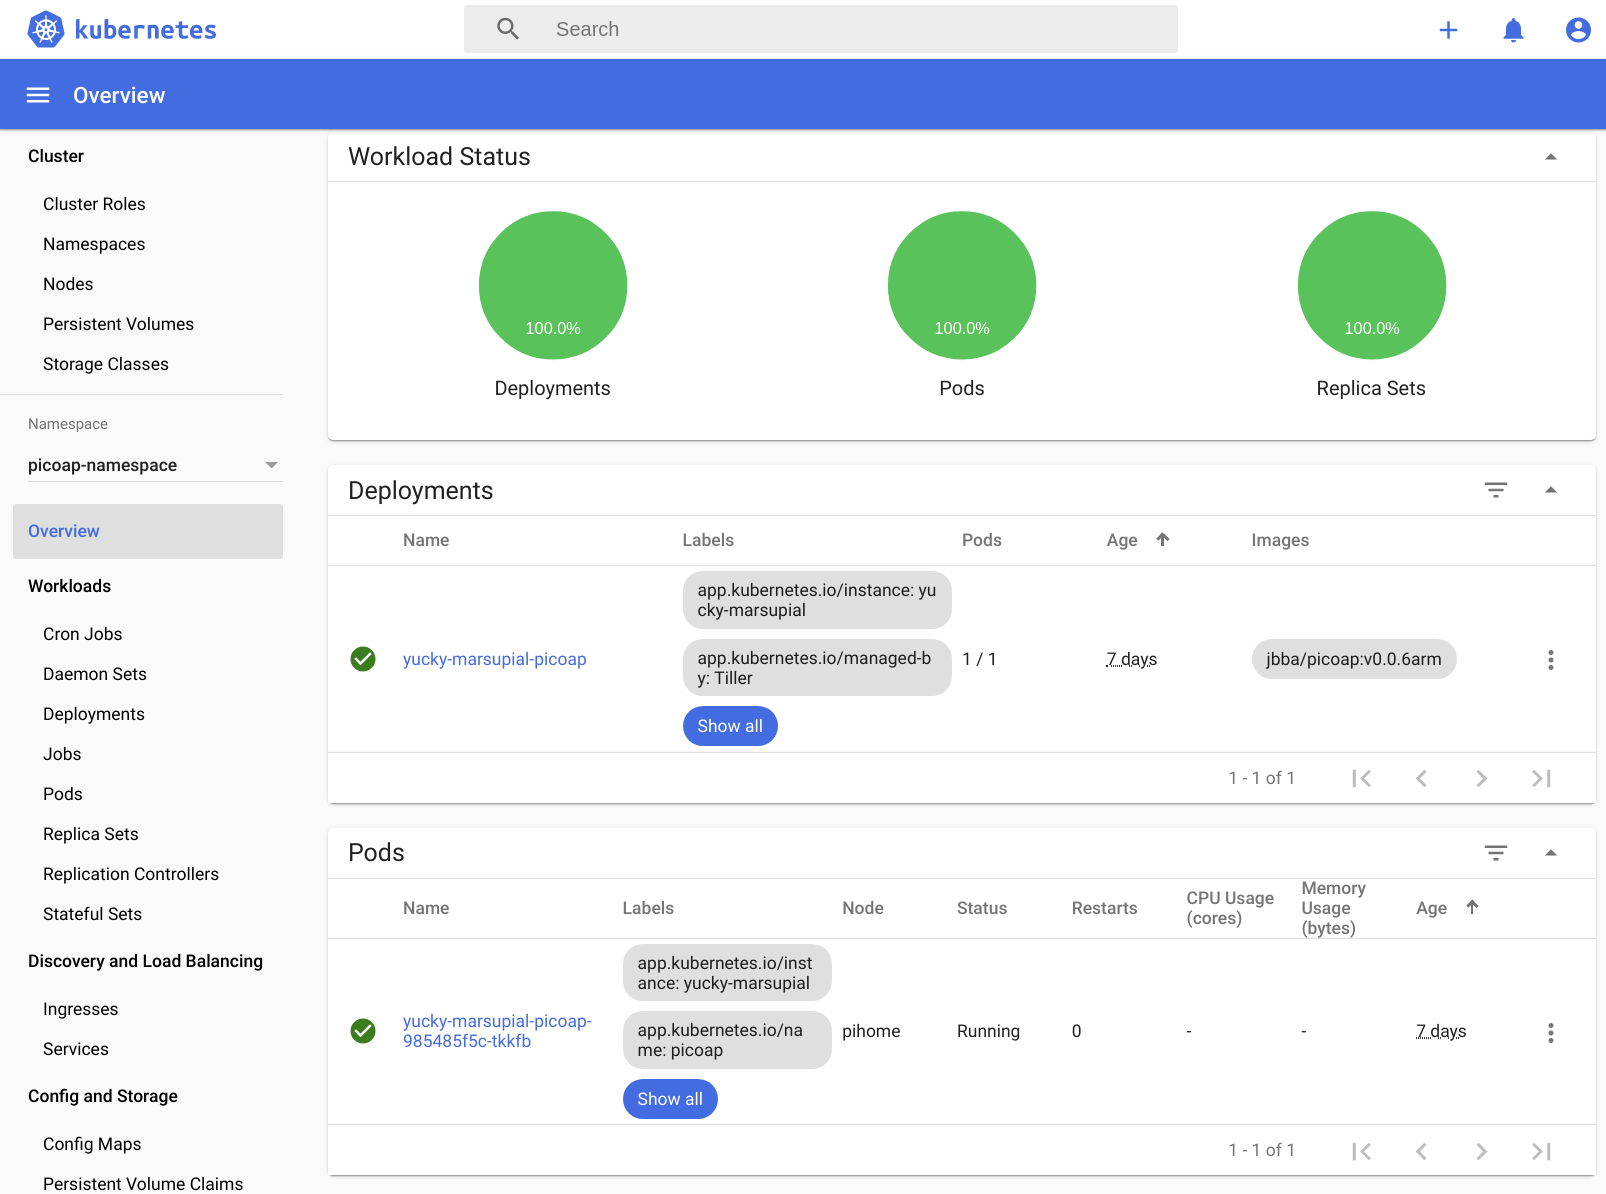
\includegraphics[width=\textwidth]{figures/dashboardK8s.png}
    \caption{The Kubernetes Dashboard showing the Edge Application.}
    \label{fig:dashboarK8s}
\end{figure}

\Cref{fig:dashboarK8s} shows the Kubernetes dashboard of the running edge application. It shows that the deployments, pods and replica sets are all working as they should. More services for the same namespace would show up here as well. To see the status of the resources in other namespaces it is enough to change to that namespace, provided the permissions are granted.

